\SourceLeaf{360}

\Needspace{17\baselineskip}
\begin{center}
[2.]
\end{center}

\begin{center}
\bfseries Centrale Projection.
\end{center}

Sind $a+bi$, $a'+b'i$ die complexen Zahlen für die Projectionen zweier Punkte, so ist von ihrer Bogendistanz

\[
\text{cosinus} = \frac{rr+aa'+bb'}{\Delta}
\]
\[
\text{sinus} = \BareRoot{\left\{[(a'-a)^2+(b'-b)^2]rr+(ab'-ba')^2\right\}}:\Delta,
\]
\[
\Delta = \BareRoot{\left\{(rr+aa+bb)(rr+a'a'+b'b')\right\}}.
\]

\begin{center}
[III.]
\end{center}

\begin{center}
\bfseries LEHRSATZ.
\end{center}

\begin{center}
\bfseries [ÜBER DIE STEREOGRAPHISCHE PROJECTION.]
\end{center}

Die wirkliche (geradlinige) Distanz zweier Punkte auf der Kugelfläche findet sich aus der Distanz ihrer stereographischen Projectionen, wenn man letztere mit dem Product der beiden Cosinus derjenigen Neigungen multiplicirt, welche die von jenen Projectionen nach dem Endpunkt einer im Centrum errichteten Normale aequal dem Durchmesser der Kugel (Halbmesser des Äquators in der Projection) gezogenen Geraden gegen die Normale haben.

\[
\text{Wirkliche Distanz} = PP'\cdot\frac{CN}{PN}\cdot\frac{CN}{P'N}.
\]

\begin{center}\resizebox{3.7cm}{!}{%
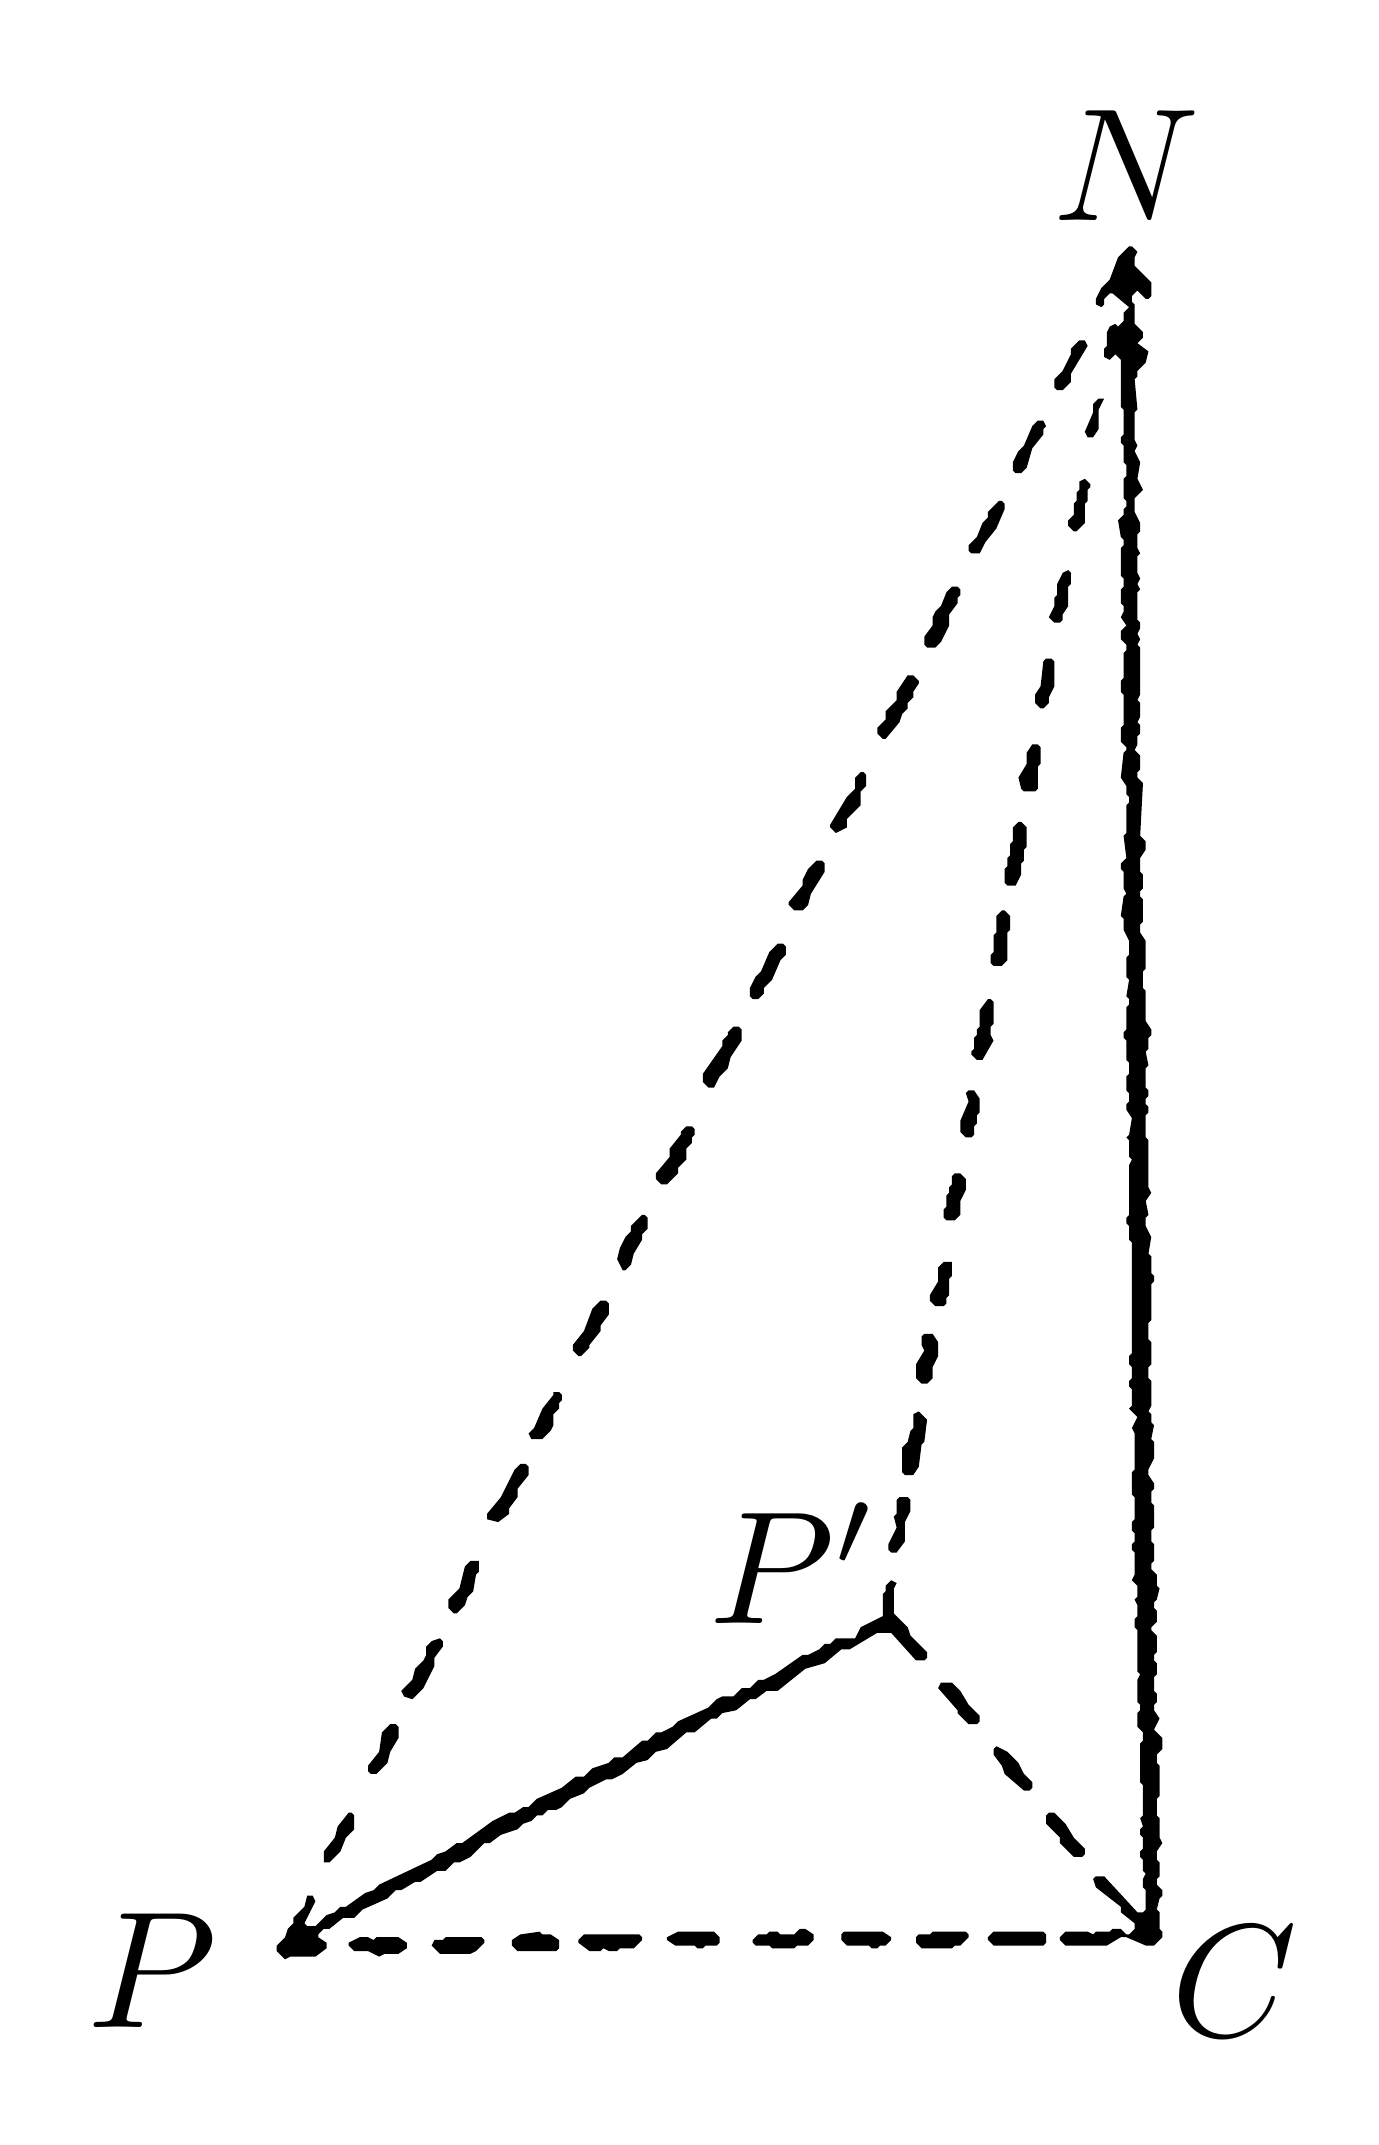
\begin{tikzpicture}[x=1pt,y=-1pt]
\path[use as bounding box] (0,0) rectangle (478,755);
\path[fill=black,draw=none,even odd rule]
(146,693) -- (149,696) -- (160,696) -- (162,695) -- (165,692) -- (165,691) -- (164,690) -- (151,690) -- (150,691) -- (147,691) -- cycle
(116,692) -- (116,693) -- (118,695) -- (123,695) -- (127,697) -- (129,696) -- (134,696) -- (137,694) -- (137,692) -- (134,690) -- (126,690) -- (125,691) -- (123,690) -- (120,690) -- cycle
(199,692) -- (203,695) -- (207,695) -- (208,694) -- (210,695) -- (213,695) -- (214,694) -- (219,694) -- (222,691) -- (222,690) -- (221,689) -- (201,689) -- (199,691) -- cycle
(347,690) -- (347,691) -- (349,693) -- (367,693) -- (368,692) -- (368,689) -- (367,688) -- (349,688) -- cycle
(321,692) -- (323,694) -- (334,694) -- (335,693) -- (337,693) -- (340,690) -- (340,689) -- (339,688) -- (327,688) -- (326,689) -- (322,689) -- (321,690) -- cycle
(294,689) -- (294,691) -- (296,693) -- (304,693) -- (305,694) -- (307,694) -- (308,693) -- (310,693) -- (312,691) -- (312,690) -- (309,688) -- (295,688) -- cycle
(231,690) -- (231,691) -- (234,693) -- (241,693) -- (242,694) -- (244,694) -- (245,693) -- (249,693) -- (250,692) -- (250,690) -- (248,688) -- (235,688) -- cycle
(175,691) -- (175,693) -- (177,695) -- (191,695) -- (192,694) -- (192,691) -- (189,689) -- (186,689) -- (185,688) -- (178,689) -- cycle
(284,689) -- (281,687) -- (279,687) -- (277,689) -- (272,689) -- (271,688) -- (268,688) -- (267,689) -- (264,689) -- (262,691) -- (262,692) -- (263,693) -- (268,693) -- (269,694) -- (277,694) -- (278,693) -- (282,693) -- (284,691) -- cycle
(369,645) -- (368,646) -- (368,649) -- (373,654) -- (373,656) -- (378,661) -- (381,661) -- (382,660) -- (382,658) -- (378,654) -- (375,649) -- (371,645) -- cycle
(117,645) -- (116,645) -- (112,650) -- (111,654) -- (107,659) -- (107,663) -- (109,663) -- (113,659) -- (115,654) -- (118,651) -- (118,646) -- cycle
(350,621) -- (349,622) -- (349,624) -- (352,628) -- (353,631) -- (360,637) -- (362,637) -- (363,636) -- (363,634) -- (360,631) -- (358,627) -- (354,623) -- cycle
(133,613) -- (131,613) -- (128,616) -- (127,623) -- (123,628) -- (123,630) -- (124,631) -- (126,631) -- (130,627) -- (131,623) -- (134,618) -- (134,614) -- cycle
(330,598) -- (329,600) -- (336,608) -- (336,609) -- (340,613) -- (343,613) -- (344,612) -- (344,610) -- (340,606) -- (337,601) -- (334,598) -- cycle
(149,582) -- (146,583) -- (144,585) -- (144,588) -- (143,590) -- (140,593) -- (139,597) -- (135,601) -- (136,603) -- (139,604) -- (143,600) -- (147,592) -- (147,589) -- (150,585) -- (150,583) -- cycle
(314,562) -- (312,561) -- (310,563) -- (310,565) -- (309,566) -- (309,574) -- (301,578) -- (299,582) -- (292,582) -- (290,584) -- (288,584) -- (286,586) -- (282,588) -- (280,588) -- (270,595) -- (266,597) -- (264,597) -- (261,600) -- (258,600) -- (255,603) -- (251,603) -- (249,604) -- (246,607) -- (235,612) -- (233,614) -- (229,616) -- (227,616) -- (224,619) -- (222,619) -- (215,625) -- (212,625) -- (210,627) -- (204,629) -- (201,632) -- (198,632) -- (193,636) -- (184,640) -- (181,643) -- (179,643) -- (176,645) -- (174,645) -- (168,648) -- (157,656) -- (155,656) -- (151,659) -- (148,660) -- (146,662) -- (127,671) -- (125,673) -- (122,674) -- (115,679) -- (113,679) -- (111,681) -- (108,682) -- (104,686) -- (101,686) -- (100,685) -- (104,677) -- (103,675) -- (101,675) -- (100,679) -- (96,683) -- (96,685) -- (94,687) -- (93,690) -- (90,693) -- (90,695) -- (93,698) -- (95,697) -- (104,697) -- (108,694) -- (108,692) -- (105,690) -- (105,689) -- (107,687) -- (109,687) -- (114,683) -- (118,683) -- (121,680) -- (130,676) -- (133,673) -- (135,673) -- (140,670) -- (142,670) -- (148,666) -- (151,666) -- (154,663) -- (156,663) -- (160,661) -- (165,656) -- (167,656) -- (171,653) -- (177,651) -- (179,649) -- (182,648) -- (184,646) -- (186,646) -- (188,644) -- (191,644) -- (193,643) -- (196,640) -- (201,638) -- (203,636) -- (209,633) -- (211,633) -- (215,631) -- (220,627) -- (224,626) -- (227,623) -- (231,622) -- (238,616) -- (241,616) -- (247,611) -- (249,611) -- (251,609) -- (256,608) -- (261,604) -- (263,604) -- (267,601) -- (271,601) -- (281,593) -- (288,591) -- (294,586) -- (297,586) -- (307,580) -- (312,580) -- (321,590) -- (324,590) -- (325,589) -- (325,587) -- (319,581) -- (318,578) -- (313,573) -- (313,564) -- cycle
(163,554) -- (160,554) -- (158,556) -- (156,564) -- (152,568) -- (152,571) -- (154,573) -- (155,573) -- (158,570) -- (159,567) -- (161,565) -- (162,559) -- (163,558) -- cycle
(318,531) -- (315,531) -- (314,532) -- (314,537) -- (313,538) -- (314,542) -- (311,548) -- (311,550) -- (312,551) -- (314,551) -- (317,547) -- (317,540) -- (319,536) -- (319,532) -- cycle
(180,519) -- (178,519) -- (176,521) -- (171,531) -- (166,537) -- (166,539) -- (170,540) -- (174,537) -- (174,535) -- (177,531) -- (177,528) -- (181,523) -- (181,520) -- cycle
(322,500) -- (320,501) -- (320,506) -- (319,507) -- (318,511) -- (316,513) -- (316,522) -- (317,523) -- (320,523) -- (322,520) -- (323,512) -- (324,511) -- (325,503) -- cycle
(192,493) -- (190,493) -- (190,494) -- (186,499) -- (183,506) -- (181,508) -- (182,510) -- (186,510) -- (189,507) -- (190,505) -- (190,501) -- (192,499) -- (192,497) -- (193,496) -- (193,494) -- cycle
(327,472) -- (324,472) -- (323,473) -- (323,476) -- (324,478) -- (321,483) -- (321,488) -- (323,490) -- (325,490) -- (327,488) -- (327,484) -- (329,480) -- (329,475) -- cycle
(209,460) -- (207,460) -- (204,463) -- (201,471) -- (197,476) -- (197,478) -- (199,480) -- (200,480) -- (203,477) -- (203,476) -- (207,471) -- (207,469) -- (210,465) -- (210,461) -- cycle
(334,446) -- (331,446) -- (329,448) -- (329,453) -- (326,458) -- (326,460) -- (328,462) -- (331,462) -- (332,461) -- (332,459) -- (333,458) -- (333,452) -- (334,451) -- cycle
(223,429) -- (222,429) -- (218,433) -- (218,435) -- (216,437) -- (214,441) -- (213,445) -- (215,449) -- (216,449) -- (218,447) -- (219,443) -- (222,438) -- (222,436) -- (224,434) -- (224,430) -- cycle
(337,414) -- (335,414) -- (334,415) -- (334,418) -- (333,419) -- (333,421) -- (332,422) -- (332,426) -- (331,427) -- (331,430) -- (332,431) -- (335,431) -- (337,429) -- (337,424) -- (339,420) -- (339,416) -- cycle
(240,397) -- (238,397) -- (236,399) -- (236,400) -- (232,405) -- (232,408) -- (227,414) -- (227,416) -- (229,418) -- (231,418) -- (235,414) -- (235,412) -- (238,409) -- (238,405) -- (240,403) -- (240,401) -- (241,400) -- (241,398) -- cycle
(342,384) -- (340,384) -- (339,385) -- (340,388) -- (337,395) -- (337,399) -- (339,401) -- (341,401) -- (342,400) -- (342,397) -- (343,396) -- (343,393) -- (344,392) -- (344,387) -- cycle
(257,361) -- (255,361) -- (253,363) -- (253,364) -- (251,366) -- (251,368) -- (244,378) -- (244,381) -- (246,383) -- (248,383) -- (250,379) -- (253,376) -- (254,372) -- (258,366) -- (258,362) -- cycle
(348,351) -- (347,351) -- (344,355) -- (344,361) -- (343,362) -- (343,364) -- (342,365) -- (342,369) -- (341,370) -- (341,371) -- (343,373) -- (345,373) -- (349,366) -- (348,364) -- (348,361) -- (349,360) -- (349,352) -- cycle
(273,331) -- (271,331) -- (268,334) -- (265,341) -- (263,343) -- (261,347) -- (261,350) -- (262,351) -- (264,351) -- (266,349) -- (266,347) -- (269,344) -- (272,337) -- (274,335) -- (274,332) -- cycle
(353,319) -- (352,319) -- (350,321) -- (350,327) -- (349,328) -- (349,334) -- (348,335) -- (348,338) -- (349,339) -- (352,339) -- (354,337) -- (354,327) -- (355,326) -- (355,321) -- cycle
(287,301) -- (285,301) -- (282,304) -- (280,308) -- (280,310) -- (275,316) -- (275,317) -- (277,319) -- (280,319) -- (282,317) -- (283,313) -- (288,305) -- (288,302) -- cycle
(359,287) -- (358,287) -- (356,289) -- (356,294) -- (355,295) -- (355,299) -- (354,300) -- (354,303) -- (353,304) -- (353,309) -- (354,310) -- (357,310) -- (359,306) -- (359,302) -- (360,301) -- (360,297) -- (361,296) -- (361,289) -- cycle
(302,269) -- (301,269) -- (299,271) -- (299,275) -- (296,278) -- (290,288) -- (290,289) -- (292,291) -- (296,289) -- (296,286) -- (301,281) -- (301,276) -- (303,274) -- (303,270) -- cycle
(365,259) -- (363,259) -- (361,262) -- (361,266) -- (358,271) -- (359,275) -- (360,276) -- (364,276) -- (365,275) -- (365,267) -- (366,266) -- (366,260) -- cycle
(320,234) -- (318,234) -- (314,240) -- (314,243) -- (310,247) -- (310,250) -- (307,253) -- (307,255) -- (309,257) -- (310,257) -- (315,251) -- (316,248) -- (318,246) -- (318,244) -- (320,242) -- (320,240) -- (322,237) -- (322,236) -- cycle
(370,228) -- (368,228) -- (367,229) -- (366,238) -- (364,241) -- (364,244) -- (366,246) -- (367,246) -- (369,244) -- (369,242) -- (371,238) -- (371,229) -- cycle
(336,202) -- (334,202) -- (332,204) -- (330,209) -- (328,211) -- (327,213) -- (327,216) -- (324,220) -- (324,223) -- (325,224) -- (328,224) -- (330,222) -- (333,216) -- (333,212) -- (336,208) -- (336,206) -- (337,205) -- (337,203) -- cycle
(376,196) -- (374,197) -- (372,201) -- (372,205) -- (371,206) -- (371,209) -- (369,213) -- (371,215) -- (373,215) -- (374,214) -- (374,212) -- (376,209) -- (376,202) -- (377,201) -- (377,197) -- cycle
(352,171) -- (351,171) -- (347,175) -- (347,177) -- (345,179) -- (343,184) -- (340,187) -- (340,189) -- (341,190) -- (344,190) -- (346,186) -- (350,181) -- (353,174) -- (353,172) -- cycle
(382,163) -- (380,164) -- (380,167) -- (379,168) -- (379,171) -- (378,172) -- (378,176) -- (376,178) -- (376,180) -- (378,182) -- (379,182) -- (382,179) -- (382,172) -- (383,171) -- (383,167) -- (384,166) -- (384,165) -- cycle
(367,142) -- (365,142) -- (363,144) -- (360,151) -- (358,153) -- (356,157) -- (356,160) -- (357,161) -- (359,161) -- (361,159) -- (363,152) -- (367,147) -- (367,145) -- (368,144) -- cycle
(389,134) -- (387,134) -- (385,136) -- (385,139) -- (382,146) -- (383,148) -- (385,148) -- (387,145) -- (387,138) -- cycle
(382,113) -- (380,113) -- (377,116) -- (377,118) -- (374,124) -- (371,127) -- (371,130) -- (372,131) -- (374,131) -- (377,128) -- (377,125) -- (383,115) -- cycle
(399,79) -- (398,79) -- (394,83) -- (391,91) -- (388,94) -- (386,98) -- (386,100) -- (388,101) -- (389,100) -- (389,98) -- (391,96) -- (392,96) -- (398,101) -- (396,103) -- (396,106) -- (394,108) -- (393,107) -- (391,108) -- (390,110) -- (390,115) -- (389,116) -- (389,119) -- (391,120) -- (393,118) -- (395,120) -- (395,137) -- (396,138) -- (396,147) -- (395,148) -- (395,150) -- (396,151) -- (396,157) -- (397,158) -- (397,162) -- (396,163) -- (396,170) -- (397,171) -- (397,173) -- (396,174) -- (396,176) -- (394,178) -- (395,184) -- (396,185) -- (396,187) -- (395,188) -- (395,198) -- (396,199) -- (396,202) -- (395,203) -- (395,208) -- (396,209) -- (396,211) -- (395,213) -- (397,216) -- (395,218) -- (395,221) -- (397,223) -- (397,225) -- (396,226) -- (396,235) -- (395,236) -- (395,240) -- (396,241) -- (396,252) -- (395,253) -- (395,258) -- (397,260) -- (397,261) -- (396,262) -- (395,271) -- (397,274) -- (397,277) -- (398,278) -- (398,280) -- (397,281) -- (397,291) -- (396,292) -- (397,300) -- (395,302) -- (395,304) -- (396,305) -- (396,311) -- (397,313) -- (396,314) -- (395,321) -- (396,322) -- (396,326) -- (398,330) -- (398,335) -- (397,336) -- (397,343) -- (398,344) -- (397,350) -- (398,351) -- (398,353) -- (397,354) -- (397,362) -- (396,363) -- (396,365) -- (397,366) -- (397,373) -- (398,374) -- (398,378) -- (397,379) -- (397,384) -- (398,385) -- (398,388) -- (397,389) -- (397,391) -- (399,394) -- (398,400) -- (397,401) -- (398,402) -- (398,408) -- (399,409) -- (398,411) -- (398,429) -- (397,430) -- (397,432) -- (398,433) -- (398,438) -- (399,439) -- (399,479) -- (398,480) -- (398,483) -- (399,484) -- (399,488) -- (398,489) -- (398,491) -- (399,492) -- (399,498) -- (398,499) -- (401,502) -- (399,506) -- (400,508) -- (400,521) -- (399,522) -- (399,530) -- (400,531) -- (400,539) -- (399,540) -- (399,543) -- (400,544) -- (400,547) -- (399,548) -- (399,550) -- (400,551) -- (400,559) -- (399,561) -- (401,563) -- (401,567) -- (400,568) -- (401,570) -- (401,574) -- (400,575) -- (400,578) -- (401,579) -- (401,594) -- (402,595) -- (401,597) -- (401,605) -- (402,606) -- (402,608) -- (401,609) -- (401,614) -- (403,616) -- (403,619) -- (402,620) -- (402,634) -- (403,635) -- (403,646) -- (402,647) -- (403,650) -- (402,651) -- (402,653) -- (403,654) -- (403,658) -- (402,659) -- (402,661) -- (403,662) -- (403,666) -- (404,667) -- (403,669) -- (403,672) -- (404,673) -- (404,680) -- (403,681) -- (401,681) -- (389,668) -- (386,668) -- (385,669) -- (386,672) -- (395,679) -- (395,681) -- (400,685) -- (400,687) -- (398,689) -- (397,689) -- (395,687) -- (392,687) -- (391,688) -- (386,688) -- (385,689) -- (383,688) -- (375,688) -- (373,690) -- (373,691) -- (375,693) -- (390,693) -- (395,690) -- (397,690) -- (404,693) -- (407,693) -- (410,690) -- (410,688) -- (409,687) -- (409,681) -- (408,680) -- (409,676) -- (410,675) -- (410,673) -- (408,671) -- (408,669) -- (409,668) -- (409,663) -- (408,662) -- (408,659) -- (410,656) -- (409,654) -- (409,647) -- (408,646) -- (408,640) -- (409,639) -- (409,628) -- (408,627) -- (408,624) -- (410,622) -- (410,618) -- (407,615) -- (409,611) -- (407,608) -- (407,606) -- (408,605) -- (408,602) -- (407,601) -- (407,596) -- (408,595) -- (408,591) -- (407,590) -- (407,588) -- (408,587) -- (408,581) -- (406,579) -- (406,578) -- (408,576) -- (408,572) -- (407,571) -- (407,569) -- (408,568) -- (409,564) -- (408,563) -- (408,559) -- (406,557) -- (406,555) -- (407,554) -- (407,548) -- (406,547) -- (406,543) -- (407,542) -- (407,534) -- (406,533) -- (406,529) -- (407,528) -- (407,526) -- (405,523) -- (405,521) -- (407,517) -- (407,511) -- (406,510) -- (407,505) -- (406,504) -- (406,501) -- (405,500) -- (406,498) -- (406,489) -- (405,488) -- (405,484) -- (406,483) -- (406,475) -- (405,474) -- (405,468) -- (406,467) -- (406,454) -- (407,453) -- (407,451) -- (406,450) -- (406,444) -- (405,443) -- (406,437) -- (404,433) -- (404,430) -- (405,429) -- (404,424) -- (406,421) -- (405,419) -- (405,402) -- (404,401) -- (404,393) -- (405,392) -- (405,390) -- (404,389) -- (404,387) -- (405,386) -- (405,384) -- (404,383) -- (404,376) -- (405,375) -- (404,370) -- (405,369) -- (405,365) -- (406,364) -- (406,362) -- (404,359) -- (404,348) -- (403,347) -- (403,341) -- (404,340) -- (404,330) -- (402,327) -- (402,324) -- (403,323) -- (403,315) -- (402,314) -- (402,312) -- (403,311) -- (403,306) -- (402,305) -- (402,300) -- (404,297) -- (404,294) -- (402,292) -- (403,273) -- (401,271) -- (401,269) -- (402,268) -- (402,263) -- (400,261) -- (401,259) -- (401,256) -- (402,255) -- (402,252) -- (401,251) -- (402,249) -- (402,244) -- (401,243) -- (402,241) -- (402,224) -- (401,223) -- (402,221) -- (401,219) -- (402,217) -- (402,215) -- (401,214) -- (401,204) -- (402,203) -- (401,201) -- (402,199) -- (401,197) -- (401,191) -- (402,190) -- (401,188) -- (401,183) -- (402,182) -- (402,179) -- (400,175) -- (400,170) -- (403,167) -- (401,163) -- (402,157) -- (400,153) -- (401,151) -- (400,149) -- (400,139) -- (401,138) -- (400,127) -- (401,126) -- (401,124) -- (404,121) -- (405,117) -- (401,114) -- (403,112) -- (403,110) -- (400,107) -- (400,100) -- (399,99) -- (399,97) -- (401,95) -- (404,98) -- (405,98) -- (406,97) -- (406,92) -- (400,86) -- (400,83) -- (401,81) -- cycle;
\node[inner sep=0pt,font=\fontsize{10}{10}\selectfont] at (397,50) {\scalebox{5.8}{$N$}};
\node[inner sep=0pt,font=\fontsize{10}{10}\selectfont] at (277,555) {\scalebox{5.8}{$P'$}};
\node[inner sep=0pt,font=\fontsize{10}{10}\selectfont] at (45,702) {\scalebox{6.0}{$P$}};
\node[inner sep=0pt,font=\fontsize{10}{10}\selectfont] at (436,706) {\scalebox{5.8}{$C$}};
\end{tikzpicture}%
}
\end{center}
\indent Man erhält so die Chorde oder eine dem Sinus des halben Bogens proportionale Grösse. Besser ist's, entweder die Projectionen durch bicomplexe Grössen $t$, $t'$ auszudrücken, wo die Distanz durch [die] Tangente des halben Bogens, gemessen durch

\[
\frac{t'-t}{1+tt'},
\]

\noindent dargestellt wird; oder sich auch der tricomplexen Grössen dabei zu bedienen.


